\hypertarget{Technologie}{\chapter{Technologie}}

\section{Požadavky}

Důležitým uvážením při tvorbě projektu byl výběr licence. Nakonec jsem se rozhodl pro použití licence GNU GPLv3, která je standardem takzvaných copyleft\footnote{Copyleft licence je typem licence pro software, který umožňuje uživatelům volně používat, upravovat a sdílet daný program, přičemž vyžaduje, aby všechny odvozené verze byly také licencovány pod stejnými podmínkami. Tím zajišťuje, že software zůstane svobodným.} licencí.

Volba licence je důležitá, protože přímo ovlivňuje, jak se dá se softwarem zacházet. GPLv3 mimo jiné zaručuje, že tento projekt navždy zůstane open-source; kdokoliv může prozkoumat, upravit a dále (pod stejnou licencí) sdílet zdrojový kód.\cite{choosealicense}

Dalšími podmínkami byly jednoduchost používání a aktuálnost různých nástrojů, programů a knihoven -- cílem bylo použít moderní (avšak osvědčené), aby program stárnul co možná nejpomaleji.

\subsection{Stack}

Dnes existuje nepřeberně způsobů jak vytvořit full-stack\footnote{Full-stack označuje kompletní řešení, často za použití serverové i klientské aplikace.} aplikaci a vybrat mezi nimi není jednoduché. Mimoto je tyto technologie potřeba často kombinovat; tato kombinace se nazývá stack. Stack určuje, jak aplikaci vyvíjíme a jaké prostředky nám jsou dostupné. Stack si můžeme vytvořit sami dle vlastního uvážení a potřeb, nebo využít nějaký volně dostupný, který už je ozkoušený a důvěryhodný.

Mojí volbou se stal \M{T3 Stack}, který kombinuje několik populárních technologií, které jsou blíže popsány níže. Zároveň je však poměrně tvárný a lze ho jednoduše přizpůsobit potřebám projektu.\cite{t3stack}

Jedno z prvních rozhodnutí, které musí člověk při tvorbě projektu udělat, je samotný výběr programovacího jazyka. Posledních pár let se většina vývoje soustředí kolem jazyka \M{TypeScript}, který je typovanou\footnote{Typy v programovacím jazyce definují struktury, ve kterých se mimo jiné dají ukládat data. Pokud předem víme, jak tyto struktury vypadají, dá se při programování lépe vyhnout chybám.} variantou jazyka \M{JavaScript}. \M{T3 Stack} ho automaticky používá. 

Framework je jakási nadstavba nad programovacím jazykem a má proces vytváření webových aplikací usnadnit. Při tvorbě webové aplikace funguje jako páteř, na které stojí vše ostatní. \M{T3 Stack} přichází s frameworkem \M{Next.js}, který je sám o~sobě nadstavbou nad populárním frameworkem \M{React}. Nabízí mnoho funkcí, jmenovitě například možnost výběru stylu renderování stránky, automatické optimalizace a~různé další funkcionality.\cite{nextjs}

% TODO: TRPC??

Databáze je další klíčovou součástí jakékoli větší aplikace. Pro tento projekt jsem zvolil \M{PostgreSQL}; jedná se o jeden z nejvšestranějších volně dostupných databázových systémů.

\M{T3 Stack} přichází s knihovnou \M{Prisma}, která komunikaci s databází usnadňuje například tím, že pro TypeScript generuje typy podle definovaného schématu.

Na rozdíl od jiných populárních CSS frameworků, jako je například \M{Bootstrap} nebo \M{Skeleton}, se \M{TailwindCSS} liší tím, že nenabízí již předem připravené komponenty, ale pouze profesionály definované CSS třídy. Vývojář díky tomu není žádným způsobem omezován.\footnote{Navíc, pokud je člověk ve tvorbě webů zběhlý, na první pohled dokáže poznat připravené komponenty z populárních CSS  frameworků, což je vzhled, kterému jsem se chtěl vyvarovat.}\cite{tailwind} \M{TailwindCSS} je automaticky obsažen v \M{T3 Stack}u.

Autentifikace je při tvorbě webových aplikací častým úskalím, proto \M{T3 Stack} automaticky přichází s \M{NextAuth.js}, což je rozšíření pro použitý framework \M{Next.js}. Umožňuje přihlašování s Google účtem, což je pro tuto aplikaci potřeba. Jedná se o léta používaný standard, což je u bezpečnostně kritického komponentu jedna~z žádaných vlastností. Zároveň jsou všechny kritické bezpečnostní chyby hlášeny na amerických státních stránkách NIST.

Sestavený kód je spouštěn pomocí \M{Node.js} za pomocí balíčkovacího programu \M{NPM}. Zároveň je možné celý program spolu s databázovým systémem spustit v \M{Docker} kontejnerech.

Program je verzován pomocí verzovacího systému \M{Git}.

Všechny výše zmíněné technologie jsou dostupné pod open-source licencemi.

\section{Program}

Program je poměrně rozsáhlý, proto je pro přehlednost rozdělen do několika souborů a složek. Všechny konfigurační soubory se nacházejí v kořenové cestě aplikace. Všechny soubory týkající se databáze, včetně migrací\footnote{Migrace je sql soubor, který definuje postupné změny databáze během vývoje.} a schématu, jsou ve složce \M{/prisma/}. Všechny statické soubory, jako jsou například obrázky a ikony, jsou ve složce \M{/public/} (toto je složka, kterou \M{Next.js} automaticky detekuje a všechny soubory uvnitř ní zveřejní v sestavené verzi aplikace). Složka \M{/src/} obsahuje samotný zdrojový kód.

\subsection{Konfigurace}
\label{sec:config}

Protože je v programu použito hodně nástrojů, je potřeba mnoha konfiguračních souborů.

\M{package.json} definuje použité knihovny a různé scripty\footnote{Script je typicky malý kus kódu, který nijak nezasahuje do funkčnosti aplikace, ale vypomáhá při jejím vývoji.}; tento soubor je vyžíván balíčkovacím systémem \M{NPM} při instalaci potřebných balíčků. \M{tailwind.config.cjs}, \M{prettier.config.cjs} a \M{postcss.config.cjs} nastavují funkčnost \M{Tailwind}u. \M{next.config.mjs} a \M{next-env.d.ts} konfigurují funkčnost \M{Next.js}. Soubor \M{.gitignore} definuje, jaké soubory má \M{Git} ignorovat.

Konfigurace samotného programu je uložena v souboru \M{.env}. Tento soubor není v~repozitáři přítomen, protože obsahuje citlivé informace (přístupové údaje k databázi aj.); místo toho je přítomen soubor \M{.env-example}, kde jsou všechny nastavitelné hodnoty popsány a nevyplněny. Níže následuje úryvek z tohoto souboru.

\begin{lstlisting}[language=Python,caption={Úryvek ukázky konfiguračního souboru programu}]
# VARIABLE INFO
NEXT_PUBLIC_SUBTITLE="Rozrazovaci testy pro [jmeno skoly]"
NEXT_PUBLIC_REPOSITORY="https://github.com/chamik/rozrazovak"
NEXT_PUBLIC_CONTACT_EMAIL="aktualni-administrator@example.org"

# Teacher email adresses (comma separated)
TEACHER_EMAILS=ucitel@gjp-me.cz,obcan-k@email.cz

# Prisma
POSTGRES_USER=postgres
POSTGRES_PASS=supertajneheslo
POSTGRES_DB=rozrazovak

# Next Auth Google Provider
GOOGLE_CLIENT_ID=
GOOGLE_CLIENT_SECRET=
\end{lstlisting}

Kvůli bezpečnosti nejsou ve výchozím stavu tyto proměnné přístupné v klientské aplikaci. Proto je potřeba k názvu těch, které na klientu chceme používat, na začátek přidat \enquote{\M{NEXT\_PUBLIC\_}}. \M{Next.js} tyto proměnné v klientské aplikaci zpřístupní.

Pro usnadnění spouštění programu lze projekt spustit v Docker kontejneru. Soubor \M{Dockerfile} definuje jak program sestavit a spustit; \M{docker-compose.yml} poté definuje, jak se má spustit databáze spolu s programem a jak mezi sebou komunikují. \cite{docker}

Script \M{start.sh} podle nastavení při každém spuštění provede migrace databáze a~konečně spouští program.

\subsection{Databáze}

Schéma databáze je definované pomocí souboru \M{prisma/schema.prisma}. Obsahuje definice uživatelů, testů, odpovědí, aktuálních přihlášení aj. (viz obrázek \ref{schema}). Jedná se o soubor se speciálním zápisem, který následně \M{Prisma} používá k vytváření SQL migrací, Typescript typů atd. Díky této funkcionalitě v programu není ani jeden ručně psaný řádek SQL kódu.

Výhodou tohoto přístupu je, že \M{Prisma} dokáže převádět tento obecný zápis a dotazy na specifické verze SQL podle použité databáze. \cite{prisma} Níže následuje úryvek schématu.

\begin{lstlisting}[language=Prisma, caption={Úryvek schématu databáze}]
model Question {
    id            Int          @id @default(autoincrement())
    languageLevel Int          @default(0)
    questionText  String       @default("")
    rightAnswer   String       @default("")
    wrongAnswers  String[]     @default(["", "", ""])
    questionType  QuestionType @default(GRAMMAR)
    pointAmount   Int          @default(1)

    answers Answer[]
}

enum QuestionType {
    GRAMMAR
    READING
    LISTENING
}
\end{lstlisting}


\begin{figure}[H]
    \centering
    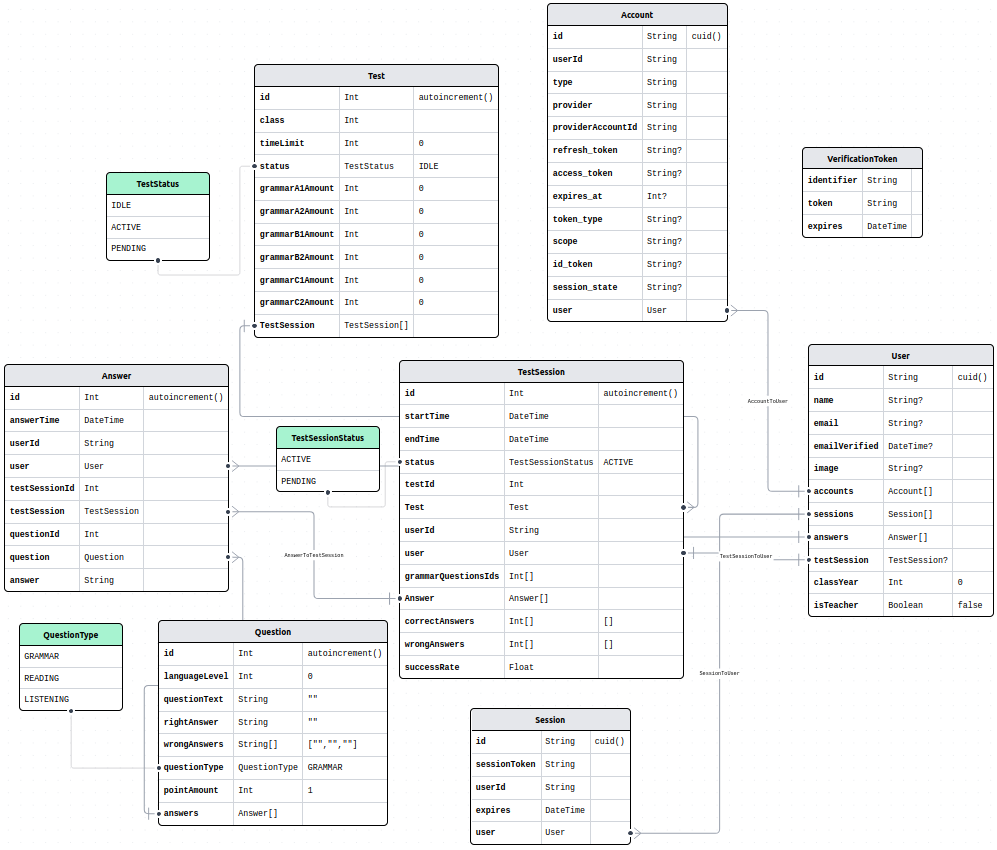
\includegraphics[width=420px]{images/02technologie/schema3.png}
    \caption{Vizualizované schéma databáze. \newline Každý blok popisuje jednu tabulku. Bloky se zeleným pruhem značí definované typy. V tabulce se nachází jména sloupců společně s jejich typy. Šedé čáry značí relace.}
    \label{schema}
\end{figure}


\subsection{Přihlašování}
\label{sec:login}

Boilerplate\footnote{Boilerplate je opakující se nebo standardní kód, který je často používán v různých částech softwaru a aplikací. Jedná se o kód, který obsahuje základní strukturu a funkce.} kód pro přihlašování přichází s \M{T3 Stack}em už připravený, je však upraven tak, aby vyhovoval požadavkům projektu -- specificky, aby aplikace umožňovala přihlašování se školním Google účtem.

Specifická implementace se nachází v \M{src/pages/api/auth/[...nextauth].ts}. \newline Při přihlášení si program kontroluje použitou e-mailovou adresu -- nejdříve pokud se nachází v seznamu učitelů (viz \ref{sec:config}), v takovém případě uživateli přidělí roli učitele s přístupem do učitelského rozhraní (viz \ref{sec:admin}). 

Pokud ne, program se ujistí, že je e-mail součástí školní domény. Díky konvenci GJP-ME dávat do emailových adres žáků rok jejich nastoupení je program schopen vypočítat jejich aktuální ročník (viz níže).

\begin{lstlisting}[language=JavaScript,caption={Zjištění aktuálního ročníku uživatele}]
function parseUserLevel(email: string) {
    const emailId = email.split('@')[0];
    
    const date = new Date();
    const currentYear = date.getFullYear();
    const currentMonth = date.getMonth();
    
    const userYear = 2000 + parseInt(emailId!.slice(0, 2)!);
    
    let level = 0
    if (emailId?.slice(2, 4) == '08')
        level = currentYear - userYear;
    else
        level = currentYear - userYear + 4;
    
    if (8 <= currentMonth && currentMonth <= 11 )
        level += 1;
    
    return level;
}
\end{lstlisting}

Aby bylo přihlašování přes Google účet možné, je potřeba svoji aplikaci registrovat v Google Developer Console. Zde lze editovat, k jakým údajům uživatele má aplikace přístup (v tomto případě pouze ke jménu a e-mailu), název aplikace zobrazený uživateli aj. Také je zde potřeba správně nastavit callback adresu -- kam Google uživatele přesměruje po přihlášení -- a potvrzené zdroje JavaScriptu.

\begin{figure}[H]
    \centering
    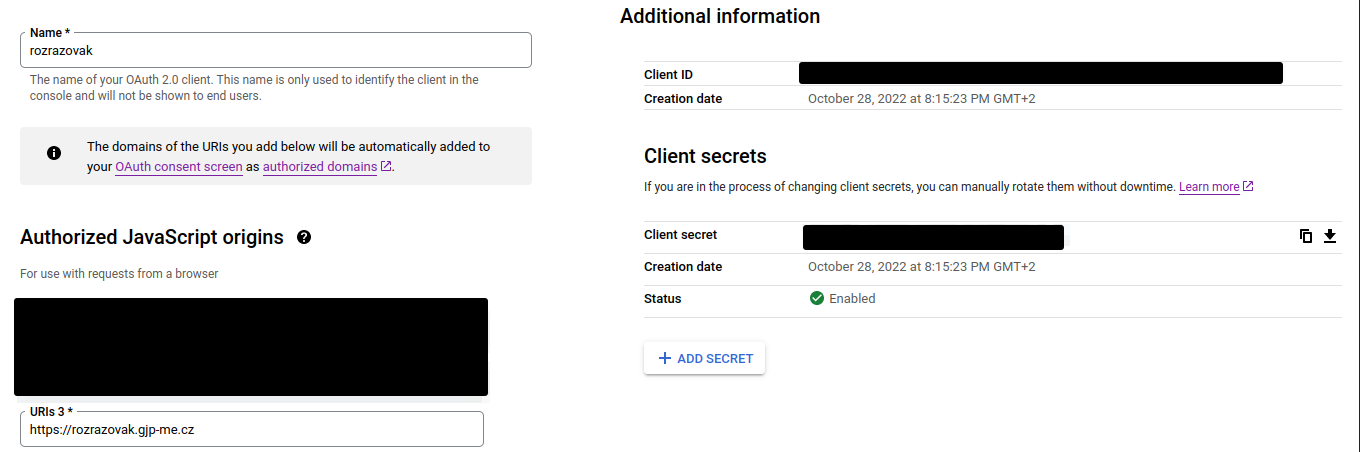
\includegraphics[width=420px]{images/02technologie/google-console.png}
    \caption{Redigovaný snímek obrazovky z Google Developer Console.}
\end{figure}

Po správném nastavení a potvrzení administrátorem organizace, podle použité domény aplikace, je na této stránce možné získat \M{CLIENT\_ID} a \M{CLIENT\_SECRET}, které je potřeba vyplnit v konfiguračním souboru aplikace (viz \ref{sec:config}).

K potvrzení identity uživatele se používá protokol \M{OAuth 2.0}, který \M{NextAuth.js} automaticky zpracuje a vývojáři zpřístupní relevantní údaje, jako je například právě e-mail a jméno.

\begin{figure}[H]
    \centering
    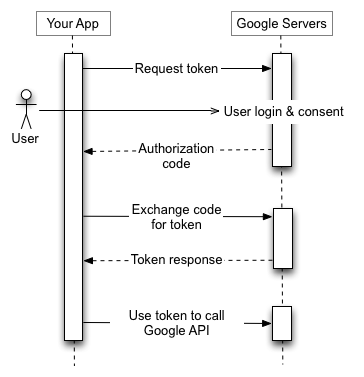
\includegraphics[width=200px]{images/02technologie/google-auth.png}
    \caption{Schéma komunikace aplikace se servery Googlu během přihlašování. Sdíleno Googlem. \cite{google-auth}}
\end{figure}

Pokud celý tento proces proběhl úspěšně, je uživatel přesměrován zpět na hlavní stránku (viz \ref{sec:login-design}). Pokud ne, uživateli je sděleno, že přihlašování neproběhlo úspěšně, a je přesměrován na interní stránku \M{NextAuth.js}, kde má možnost se zkusit přihlásit znovu.

\section{API}
\label{api}

Přestože se celý program zapisuje do jedné souborové struktury, běží některý kód pouze na serveru. Tyto funkce se nachází v \M{/src/server/}. \M{Next.js} při kompilaci spojí všechny typescript zdrojové soubory a vytvoří z nich jeden javascript program. Tento program spustí svůj webserver na portu definovaném v konfiguraci (viz \ref{sec:config}). API\footnote{API (application programming interface; česky rozhraní pro programování aplikací) definuje možnosti vzájemné komunikace aplikací (v tomto případě serveru a klienta).} samotné je dostupné na cestě \M{[doména]/api/trpc/} -- tato adresa je definována v \M{/src/utils/tprc.ts} a je na ni možné posílat tradiční \M{json} požadavky. Toto API využívá v pozadí i aplikace.

API je rozdělené do dvou hlavních částí s různými pravomocemi -- uživatelské a učitelské. Uživatelské je dostupné všem přihlášeným uživatelům. Učitelské je dostupné pouze oprávněným uživatelům -- server si zkontroluje, pokud je u uživatele v databázi vyplněná kolonka \M{isTeacher}. Tento kód se nachází v \M{/src/server/trpc/trpc.ts} a jeho ukázka je níže.

\begin{lstlisting}[language=JavaScript,caption={Kontrola přístupu do učitelského rozhraní}]
const isTeacher = t.middleware(async ({ ctx, next }) => {
    if (!ctx.session || !ctx.session.user) {
        throw new TRPCError({ code: "UNAUTHORIZED" });
    }
    
    const user = await ctx.prisma.user.findFirst({ where: 
        { email: ctx.session.user.email }});

    if (!user || !user.isTeacher)
        throw new TRPCError({ code: "UNAUTHORIZED" });
    
    return next({
        ctx: {
        // infers the `session` as non-nullable
        session: { ...ctx.session, user: ctx.session.user },
        },
    });
});

export const teacherProcedure = t.procedure.use(isTeacher);
\end{lstlisting}

\subsection{Uživatelské API}
\label{userapi}

Uživatelské API se nachází v \M{/src/server/trpc/router/user.ts}. Definuje následující endpointy\footnote{API endpoint je specifický koncový bod nebo URL v rámci API, který představuje konkrétní operaci nebo zdroj poskytovaný daným rozhraním. V tomto případě každý endpoint reprezentuje jednu funkci na serveru.}:

% TODO: tečky na konci řádků?
\begin{compactitem}
    \item getUserData -- vrátí informace o přihlášeném uživateli, aktuálním spuštěném testu a případně o vyplněném testu;
    \item beginTest -- vygeneruje test pro daného uživatele, uloží do databáze ID použitých otázek a čas ukončení testu ;
    \item getTestData -- navrátí náhodně zamíchaná vygenerovaná data testu, označí test za aktivní;
    \item submitAnswer -- přijímá odpověď na otázku, kterou uloží do databáze;
    \item submitTest -- potvrdí odevzdání testu, zablokuje další odevzdávání otázek, zároveň test vyhodnotí a výsledky uloží do databáze.
\end{compactitem}

Následuje ukázka endpointu \M{getTestData}.

\newpage
\begin{lstlisting}[language=JavaScript,caption={Endpoint getTestData}]
getTestData: protectedProcedure.query(async ({ ctx }) => {
    const user = await prisma.user.findFirst({ 
        where: { email: ctx.session.user.email },
    });

    if (!user)
        return;

    const sesh = await prisma.testSession.findFirst({
        where: { userId: user.id },
    })

    if (!sesh)
        return;

    const questionsIds = sesh.grammarQuestionsIds;
    const questions = await prisma.question.findMany({
        where: {
            id: { in: questionsIds }
        },
        select: {
            id: true,
            questionText: true,
            rightAnswer: true,
            wrongAnswers: true,
        },
    });

    const shuffled = shuffle(questions.map(x => ({
        id: x.id,
        questionText: x.questionText,
        answers: shuffle([x.rightAnswer, ...x.wrongAnswers]),
    })));

    const answers = await prisma.answer.findMany({
        where: {
        testSessionId: sesh.id,
        },
        select: {
        questionId: true,
        answer: true,
        },
    });

    return ({
        questions: shuffled,
        testSession: sesh,
        submittedAnswers: answers,
    });
}),
\end{lstlisting}

\newpage
\subsection{Učitelské API}
\label{adminapi}

Učitelské API se nachází v \M{/src/server/trpc/router/admin.ts}. Definuje následující endpointy:

\begin{compactitem}
    \item getAllQuestions -- navrátí obecné informace o všech otázkách v databázi;
    \item getQuestionById -- získá detail otázky z databáze podle daného ID;
    \item getTestById -- získá detail testu z databáze podle daného ID;
    \item saveQuestion -- uloží nové údaje po editaci otázky do databáze;
    \item newQuestion -- vytvoří novou otázku s výchozími údaji a uloží ji do databáze;
    \item getQuestionLevels -- vrátí počet otázek v databázi pro každou jazykovou obtížnost;
    \item deleteQuestion -- odstraní otázku z databáze;
    \item getAllTests -- navrátí obecné informace o všech testech v databázi;
    \item saveTest -- uloží nové údaje po editaci testu do databáze;
    \item deleteTest -- odstraní test z databáze (tento endpoint nelze spustit manuálně přes uživatelské rozhraní, používá se pouze interně);
    \item toggleTest -- označí test jako \M{AKTIVNÍ}, nebo \M{VYPLNĚNÝ}, podle jeho aktuálního stavu;
    \item restartTest -- ze stavu \M{VYPLNĚNÝ} nevratně smaže data o vyplnění a vrátí ho do stavu \M{VYPNUTÝ};
    \item areTestRunning -- vrátí pravdivostní hodnotu, pokud je alespoň jeden test ve stavu \M{AKTIVNÍ}, nebo \M{VYPLNĚNÝ};
    \item downloadResults -- vygeneruje excel tabulku, do které přidá data výsledků daného testu, a vrátí ji převedenou do formátu Base64.
\end{compactitem}

Následuje kód pro endpoint \M{downloadResults}.

\begin{lstlisting}[language=JavaScript,caption={Endpoint downloadResults}]
downloadResults: teacherProcedure.input(z.object({testId: z.number()})).mutation(async ({ input }) => {
    const test = await prisma.test.findFirst({ where: { id: input.testId }});
    if (!test) return;
    
    if (test.status != TestStatus.PENDING) return;

    const results = await prisma.testSession.findMany({
      where: {
        testId: input.testId,
      }, 
      orderBy: {
        successRate: "desc",
      }
    });

    if (!results) return;

    const users = await prisma.user.findMany({
      where: {
        id: {
          in: results.map(x => x.userId),
        }, 
      },
    })

    const workbook = new Workbook();
    const worksheet = workbook.addWorksheet('Vysledky testu')

    worksheet.columns = [
      { header: "Jmeno", key: "name", width: 25 },
      { header: "E-mail", key: "email", width: 30 },
      { header: "Body gr.", key: "points_gr", width: 10},
      { header: "Uspesnost gr.", key: "success_gr", width: 15 },
      { header: "ID spatnych odpovedi gr.", key: "wrong_ids_gr", width: 40 },
    ];

    const usrs = users.reduce((acc, user) => {
      acc[user.id] = user;
      return acc;
    }, {} as { [key: string]: typeof users[0] });

    results.forEach(s => {
      worksheet.addRow({
        name: usrs[s.userId]?.name ?? "Bezejmenny",
        email: usrs[s.userId]?.email ?? "???",
        points_gr: s.correctAnswers.length,
        success_gr: (s.successRate * 100).toFixed(1) + "%",
        wrong_ids_gr: s.wrongAnswers.join(" "),
      });
    });

    const bf = await workbook.xlsx.writeBuffer();
    const st = Buffer.from(bf).toString("base64");

    return st;
}),
\end{lstlisting}

\newpage
\section{Komponenty a stránky}

Většinu programu tvoří komponenty a stránky knihovny \M{React}. Jedná se vlastně o~TypeScript soubor doplněný o prvky HTML, které se zobrazují v prohlížeči. Komponenty se nacházejí v \M{/src/components/}, stránky v \M{/src/pages/}. Níže následuje několik různých ukázek komponent a stránek použitých v aplikaci. 

Zobrazení stavu testu podle aktuální hodnoty. V argumentech \M{className} HTML tagů lze vidět třídy \M{TailwindCSS}.

\begin{lstlisting}[language=JavaScript,caption={Úryvek z \M{/src/pages/admin/tests/index.tsx}; Status testu}]
type TestBadgeProps = {
    status: TestStatus,
}

const TestBadge: React.FC<TestBadgeProps> = (props) => {
    const {
        status,
    } = props;

    if (status == TestStatus.ACTIVE) return (
        <p className="text-2xl font-bold text-green-600">
            AKTIVNI
        </p>
    )
    else if (status == TestStatus.IDLE) return (
        <p className="text-2xl font-bold text-red-600">
            VYPNUTY
        </p>
    )
    else return (
        <p className="text-2xl font-bold text-yellow-500">
            VYPLNENY
        </p>
    )
}
\end{lstlisting}

\newpage
Při vyplňování textu otázky (viz obrázek \ref{questionfill}) lze použít znak podtržítka \enquote{\_}, který se v textu otázky při vyplňování zobrazí jako světle fialový obdélník (viz obrázek \ref{purplerect} u druhé otázky), který uživateli naznačuje, že se na dané místo má něco doplnit. 

\begin{lstlisting}[language=JavaScript,caption={Úryvek z \M{/src/pages/test/index.tsx}; komponent textu otázky, výměna znaku \enquote{\_} za fialový obdélník}]
type QuestionTextProps = {
    questionText: string,
    id: number,
}

const QuestionText: React.FC<QuestionTextProps> = (props) => {
    const {
        questionText,
        id,
    } = props;

    const ar = questionText.split("_");
    return(
        <div className="flex flex-row justify-between"> 
            <h3 className="font-bold text-lg mb-3 my-auto">
                {...intersperse(ar, (<span className="w-14 inline-block rounded-lg bg-purple-100 border-2 border-purple-200 mx-1 text-transparent">___</span>))}
            </h3>
            <p className="w-20 my-auto text-slate-300 hover:text-black hover:font-semibold mx-2">id: {id}</p>
        </div>
    )
}
\end{lstlisting}

\newpage
\begin{lstlisting}[language=JavaScript,caption={Úryvek z \M{/src/pages/admin/grammar/index.tsx}; generování seznamu otázek z databáze}, label={xslxgen}]
type QuestionsListingProps = {
    questions: Question[] | undefined,
    getQuestionDataCallback: (id: number) => void,
};

const QuestionsListing: React.FC<QuestionsListingProps> = (props) => {
    const {
        questions,
        getQuestionDataCallback
    } = props;

    if (!questions) return (
        <>
        </>
    );

    return (
        <>
            {questions.map(question => (
                <Link href={`/admin/grammar/?id=${question.id}`} key={question.id} onClick={() => getQuestionDataCallback(question.id)}>
                    <div className="flex justify-start px-8 py-2 mb-2 text-left text-slate-700 hover:ring-2 ring-purple-600 rounded-3xl hover:cursor-pointer font-extrabold">
                        {/* <p className="w-10 mr-4">{question.id}</p> */}
                        <p className="w-96 mr-4 truncate">{question.questionText}</p>
                        <p className="w-80 mr-4 truncate">{question.rightAnswer}</p>
                        <p className="w-40 mr-4">{numToLevel(question.languageLevel)}</p>
                        <p className="w-10 mr-4 text-slate-400">{question.id}</p>
                    </div>
                </Link>
            ))}
        </>
    );
}
\end{lstlisting}